\section{Maximal equicontinuous factor}
\subsection{Definition, $\exists!$, universal property}
\begin{frame}
  Let $(X,T)$ be a TDS.
  \begin{definition}[Maximal equicontinuous factor (MEF)]
    A factor $\pi : (X,T) \to (Y,T)$ is called a \emph{MEF} of $(X,T)$ if and only if
  \begin{itemize}
    \item $\pi$ is equicontinuous,
    \item $\pi$ is maximal, i.e. $\forall \varphi : (X,T) \to (Y,T)$ equicontinuous factor: $R_\pi \subset R_\varphi$.
  \end{itemize}
\end{definition}
\pause
  \begin{alertblock}{Theorem (Existence and uniqueness of the MEF)}
  Let $(X,T)$ be a TDS.
  Then $(X,T)$ has a MEF and any two MEF's are equivalent.
  \end{alertblock}
  \pause
\begin{example}[MEF of equicontinuous TDS is trivial]
  $(X,T)$ equicontinuous, then $I: (X,T) \to (X,T)$ is the MEF of $(X,T)$.
\end{example}

\end{frame}
\begin{frame}[fragile]
\begin{proposition}[Universal property of the MEF]
  Let $\pi : (X, T) \to  (X_m,T)$ be the MEF.
  Then:
  \begin{equation*}
    \forall \, \varphi : (X,T) \to (Y,T) \ \text{equicontinuous factor} \ \exists!\tilde{\varphi}: (X_m,T) \to (Y,T): \varphi = \tilde{\varphi} \circ \pi.
  \end{equation*}
  \end{proposition}
  \begin{center}
    \begin{tikzcd}[sep=large]
      (X,T) \arrow[d, "\pi"'] \arrow[r, "\varphi \ \text{equic.}"]  \arrow[dr, phantom, "\circlearrowleft", near start] 
      & (Y,T) \\
      (X_m,T)  \arrow[ur,"\exists ! \tilde{\varphi}"'] & \phantom{a} \\
    \end{tikzcd}
  \end{center}
\end{frame}
\subsection{Eigenfunction characterisation of the MEF}
\begin{frame}
  $(X,T)$ TDS with $T$ abelian, $T^*$ the set of all (continuous) characters of $T$.
\begin{definition}[Koopman operator]
  \begin{equation*}
    \begin{split}
      &U : T \longrightarrow L(C(X)) \\
      &(U(t) f)(x) := f(t^{-1}x).
    \end{split}
  \end{equation*}
   \end{definition}
   \pause
   \begin{definition}[Eigenvalue, Eigenfunction]
   \begin{equation*}
    \begin{split}
      &0 \neq f \in C(X) \ \text{\emph{eigenfunction} of} \ U \ \text{to \emph{eigenvalue}} \ \chi \in T^*   \\
 &:\Leftrightarrow f \in \ker (U-\chi):= \bigcap_{t \in T} \ker (U(t)- \chi (t)I).
    \end{split}
      \end{equation*}
   \end{definition}
\end{frame}
\begin{frame}[fragile]
 \begin{definition}[Discrete spectrum]
  \begin{equation*}
    (X,T) \ \text{has \emph{discrete spectrum}}:\Leftrightarrow C(X) = \overline{\lin} \bigcup_{\chi \in T^*} \ker (U- \chi).
  \end{equation*}
\end{definition}
\pause 
  \begin{alertblock}{Theorem}%
  \begin{equation*}
    (X,T) \ \text{is equicontinuous} \Leftrightarrow (X,T) \ \text{has discrete spectrum}
  \end{equation*}

    \hfill(see \cite{HK2023}, Theorem 2.11)
\end{alertblock}
\pause
  \begin{alertblock}{Theorem (MEF eigenfunction characterisation)}
  \label{thm:MEF_EFchar}
  Let $x_1,x_2 \in X$. Let $\pi : (X,T) \to (X_m,T)$ be the MEF.
  Then
  \begin{equation*}
  \pi (x_1) = \pi (x_2) \Leftrightarrow 
    \forall f \in \bigcup_{\chi \in T^*} \ker (U- \chi) : f(x_1) = f(x_2).
  \end{equation*}
\end{alertblock}
\end{frame}
\begin{frame}
  \begin{columns}
    \begin{column}{0.6\textwidth}
    \centering
      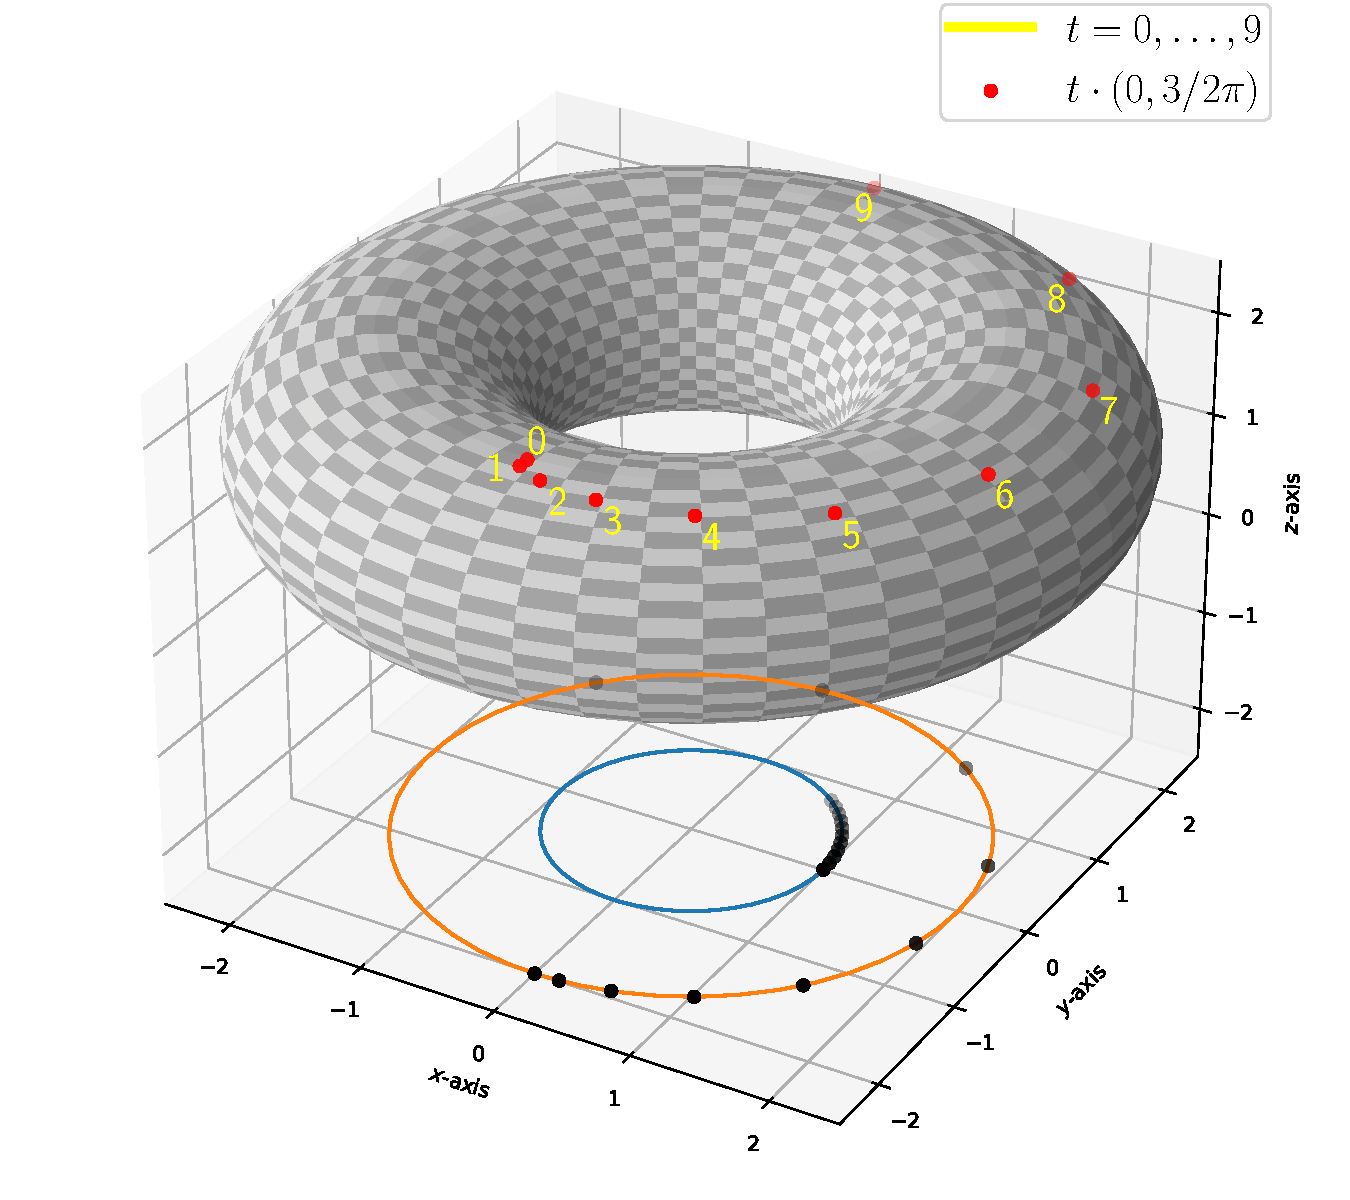
\includegraphics[width=8cm]{imgs/torusSkewRot.pdf}
    \end{column}
    \begin{column}{0.4\textwidth}
  \begin{example}[MEF of skew rotation]
Let $a \in \mathbb{T}$. Homeomorphism:
\begin{equation*}
  \begin{split}
    &\alpha: \mathbb{T}^2 \to \mathbb{T}^2,\\
  &\alpha (z,w) := (az,zw).
  \end{split}
  \end{equation*}
     TDS $(\mathbb{T}^2,\mathbb{Z})$, $\mathbb{Z}$-action:
     \begin{equation*}
     t \cdot (z,w) := \alpha^t (z,w).
     \end{equation*}
     \pause
  MEF is 
  \begin{equation*}
    \begin{split}
     &\pr_1 : (\mathbb{T}^2,\mathbb{Z}) \to (\mathbb{T},\mathbb{Z}), \\
    &\pr_1 (z,w) := z.
    \end{split}
  \end{equation*}
  $\mathbb{Z}$-action on $\mathbb{T}$:
  \begin{equation*}
   t\cdot  z := a^tz.
  \end{equation*}
\end{example}
       \end{column}
  \end{columns}
\end{frame}
\subsection{Relationship of MEF and Kronecker factor}
\begin{frame}
  ... to be continued
\end{frame}

